\section{Fit Strategy and Validation}
\label{sec:fit_strategy}

The steps taken to validate the fitting approach for both the SVJ Fit strategy and the Discovery strategy will be outlined in the following sections. The signal region fits which comprise the final result will be presented in Chapter~\ref{ch:results}.

\subsection{SVJ Fit Strategy}
\label{subsec:fit_exclusion}

The ability of the five parameter fit function to capture the shape of the background is studied extensively, using data from the CR and VR. Signal injection tests are performed to determine the ability of the fit to recover and quantify any SVJ signal excess. Estimates of the expected sensitivity and the ability to set upper limits on the cross-section of the signal process are also verified.
%Results: An overview of the final fit setup including the final discriminating variables(s), the (SR/CR) regions to be included in the fit and the floating normalization parameters. 
%Some rough first expected limits/discovery sensitivity plots are useful if you have them but not necessary. In this case the binning of the final variable(s) and the systematics smoothing/pruning should be indicated.


%------------------------------------------------- 
\subsubsection{Background Only Fits}
\label{subsec:fit_bkgonly}

Three validations are used for the background fit polynomial: MC across all analysis regions, data in the CR and VR, and pseudo-data in the CR and VR. 

Figure~\ref{fig:bkgfit_mc} shows the ability of this polynomial to fit the smoothly falling \mt~background in simulation across all 3 analysis regions (CR, VR, SR).
The \mt~spectrum is fit in 90 even bins.
These distributions are obtained by downsampling the MC statistics to match the relevant statistics of the data region, in accordance with the MC weights.
The high background-only $p$-value indicates a good fit.
\begin{figure}[!htbp]
\centering
   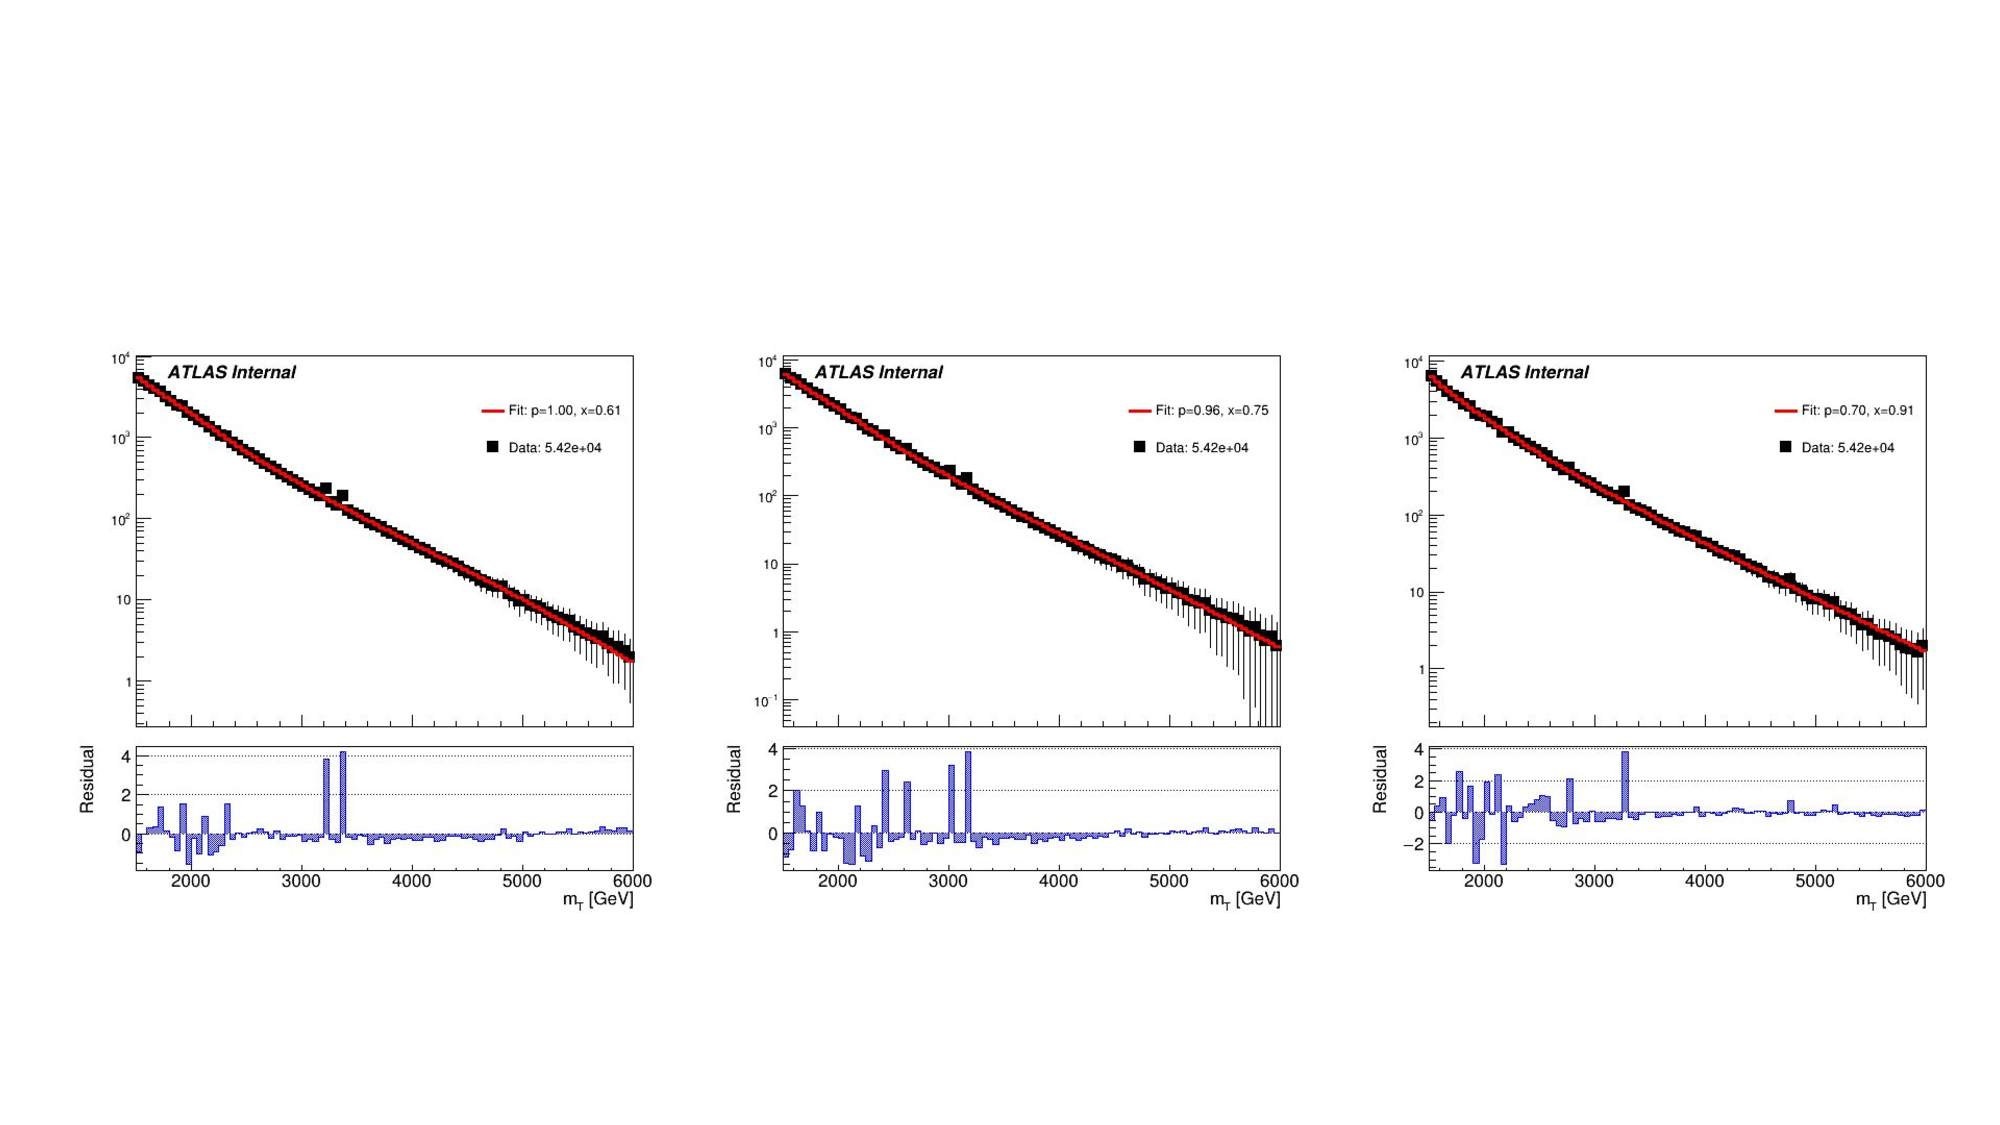
\includegraphics[width=0.95\textwidth]{figures/stats/bkgfit_mc}
    \caption{Background-only \mt~fits using representative MC in the CR (left), VR (middle), and SR (right).
    \label{fig:bkgfit_mc}}
\end{figure}

A slight sinusoidal pattern in the residuals may be observed. 
This arises due to the ``stitching" of the \pt~slices for the QCD MC (as shown in Figure~\ref{fig:jzslices}), which is picked up by the fit.
For this reason, fitting to MC is only checked to verify that the differences in the slope of \mt~between the three regions (as shown in Figure~\ref{fig:crvrsr_mt}) do not pose a problem for the fitting strategy.

The nature of the functional fitting method allows it to easily adapt to changes in slope of a smoothly falling distribution.
Thus validation of the fit can be performed in data using the CR and the VR distributions to model the expected behavior in the SR. 
Figure~\ref{fig:bkgfit_data_fullstats} shows the a successful fit performed on the full statistics CR and VR regions.
\begin{figure}[!htbp]
\centering
   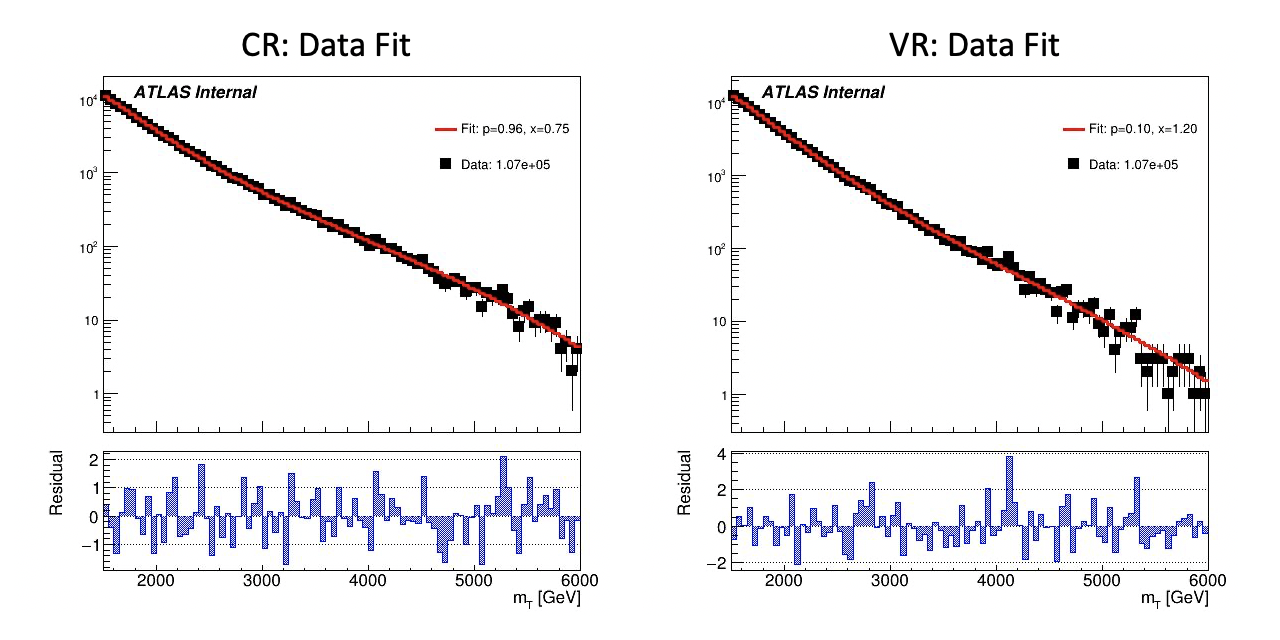
\includegraphics[width=0.8\textwidth]{figures/stats/bkgfit_data_fullstats}
    \caption{Background-only \mt~fits using data in the full statistics CR and VR regions.
    \label{fig:bkgfit_data_fullstats}}
\end{figure}

Table~\ref{fig:postfit_param_pfn} shows the post-fit values of the fit parameters and their uncertainties for each fit. 
\begin{table}[!htbp]
\centering
   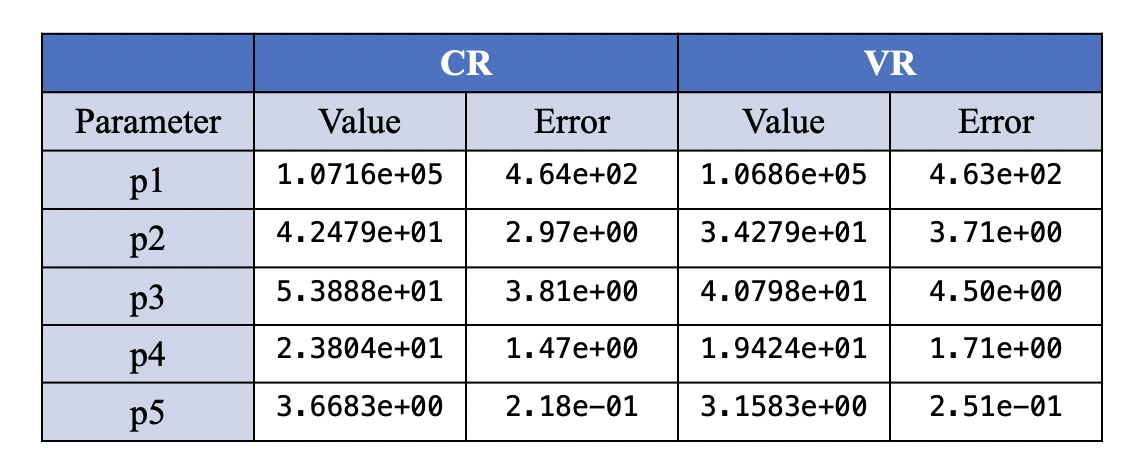
\includegraphics[width=0.75\textwidth]{figures/stats/postfit_param_pfn}
    \caption{Post-fit parameters for the PFN CR and VR. $p1$ can also be considered $N_{bkg}$ or the normalization factor.
    \label{fig:postfit_param_pfn}}
\end{table}

To further validate the fit stability of the fit against potential statistical fluctuations, \textit{pseudo-data} (also known as \textit{toy datasets}) are created from the CR data distribution. 
The pseudo-data is created following an \textit{Asimov} prescription \cite{asimov}, using a template to generate a set of toys representing different possible statistical fluctuations.
When studied as a group, the performance of the pseudo-data collection represents the range of possible behavior for an unknown distribution (the SR data in this case), given its statistical uncertainties.

The template used to generate the pseudo-data is a \textit{smoothed} and \textit{scaled} version of the CR. 
The smoothing applied follows the procedure for functional decomposition described in Ref.~\cite{edgar2018functional}.
Figure~\ref{fig:smoothing} shows the impact of smoothing on the source data distribution in the CR.
\begin{figure}[!htbp]
\centering
   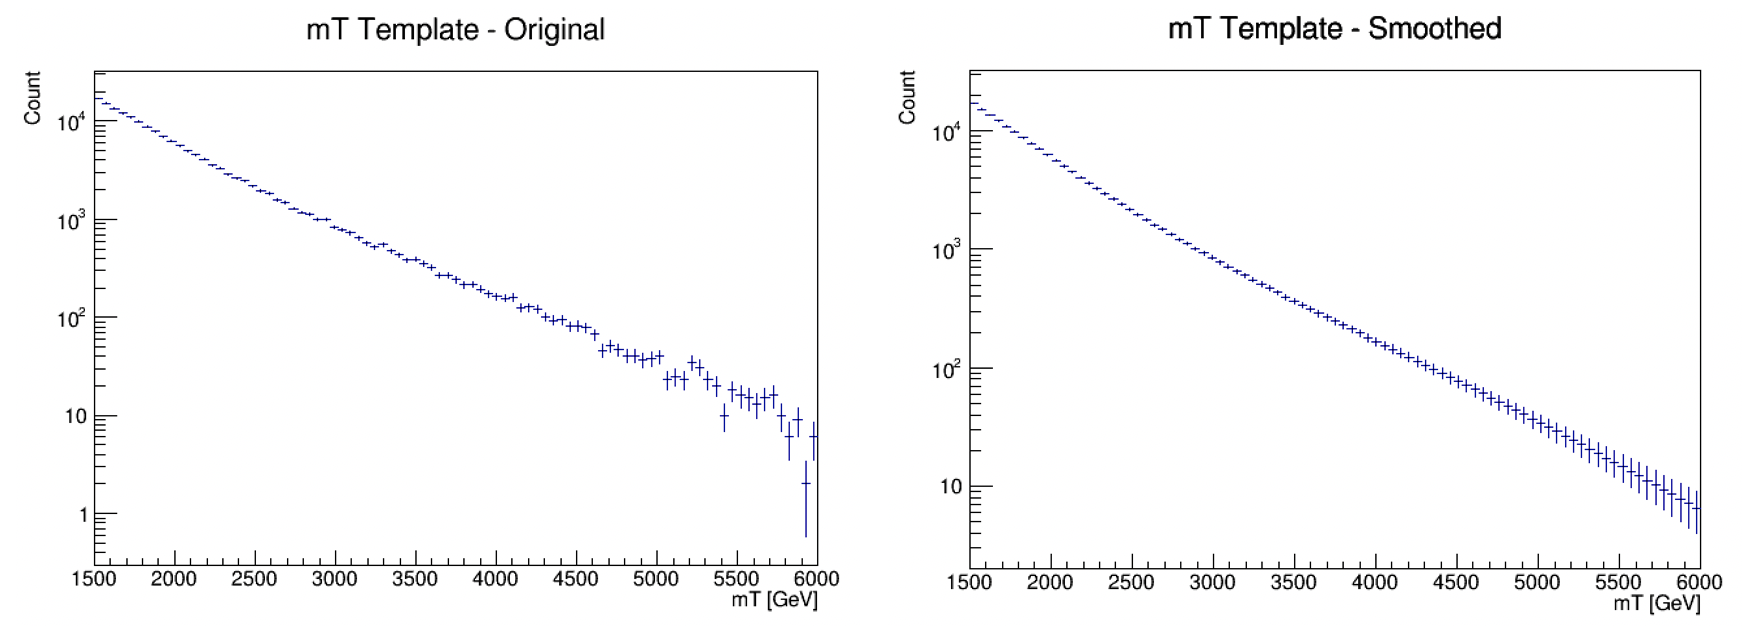
\includegraphics[width=0.95\textwidth]{figures/stats/smoothing}
    \caption{\mt~distribution in the data CR, before (left) and after (right) smoothing.
    \label{fig:smoothing}}
\end{figure}

The scaling adjusts the statistics of the smoothed template to the expected statistics of the SR.
Recall Figure~\ref{fig:crvrsr_2d}, which illustrates that the statistics of the CR and the VR are almost 3x the expected statistics of the SR.
The polynomial fitting strategy is sensitive to the statistics of the fitted template, so its performance can very substantially depending on the statistical power of the fitted distribution.
To mitigate this, the smoothed template is scaled to the expected statistics of the SR.
Toys are then generated from the smoothed distribution, by varying each bin within its statistical uncertainty according to a Poisson distribution. 
Each toy has the same statistical power as the SR, within statistical uncertainly.

Figure~\ref{fig:bkgfit_data} shows example fits to three such toy datasets.
Figure~\ref{fig:asimov_hist} shows the resulting p-values after an ensemble of 100 Asimov pseudo-datasets are each individually fit. 
This test determines the likelihood of exceptionally good (high p-value) or poor (low p-value) fits due to randoms statistical fluctuations in the data. 
A flat distribution is observed, indicating good statistical behavior. 

\begin{figure}[!htbp]
\centering
   %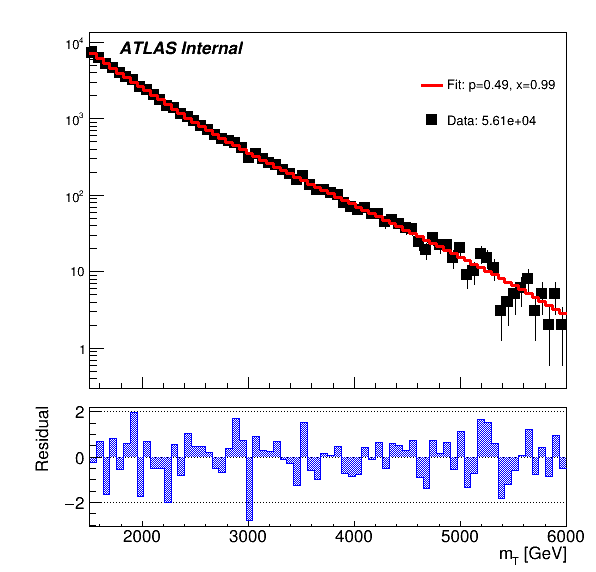
\includegraphics[width=0.32\textwidth]{figures/stats/dataDSfiveParFitChi2_CR0.png}
   %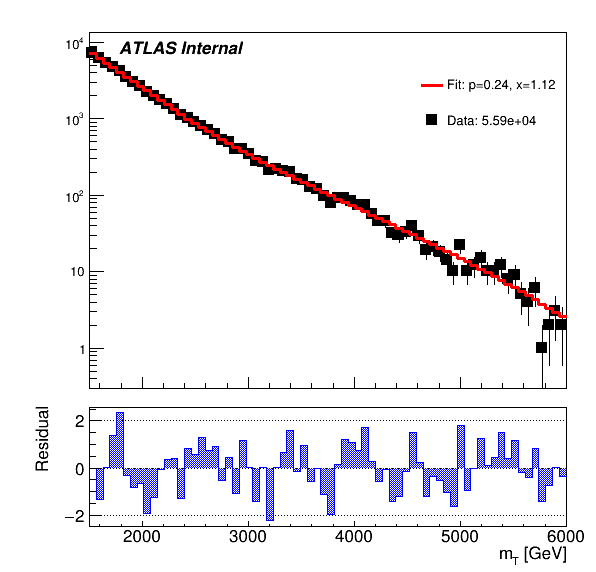
\includegraphics[width=0.32\textwidth]{figures/stats/dataDSfiveParFitChi2_CR1.png}
   %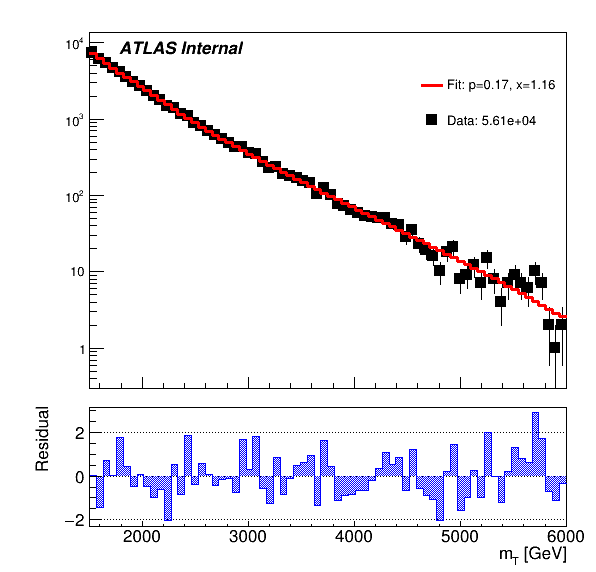
\includegraphics[width=0.32\textwidth]{figures/stats/dataDSfiveParFitChi2_CR2.png}
   %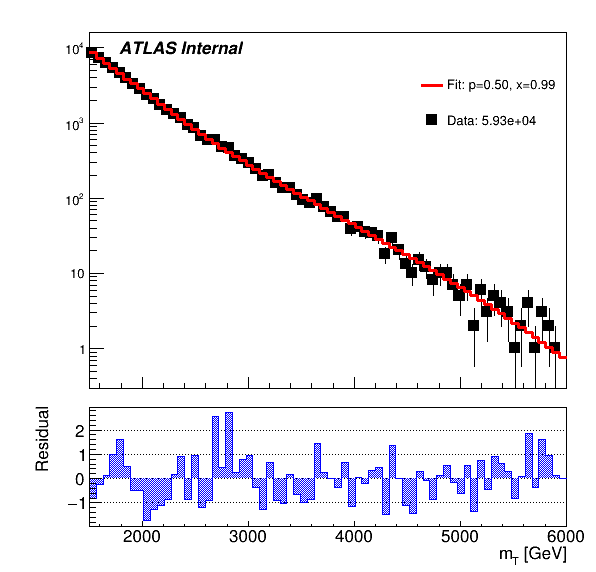
\includegraphics[width=0.32\textwidth]{figures/stats/dataDSfiveParFitChi2_VR0.png}
   %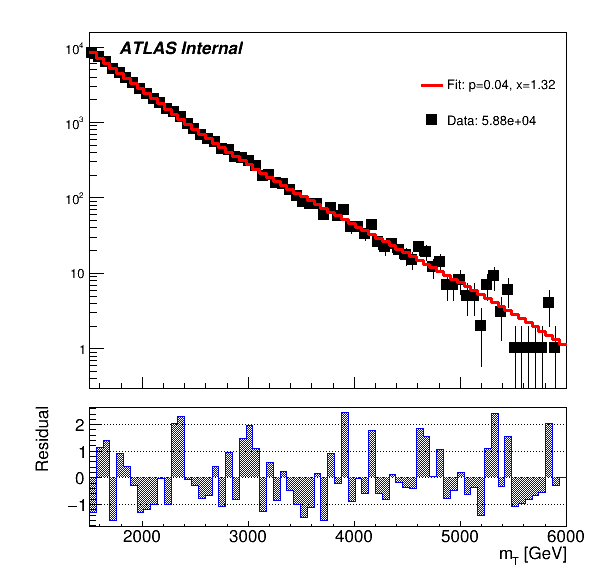
\includegraphics[width=0.32\textwidth]{figures/stats/dataDSfiveParFitChi2_VR1.png}
   %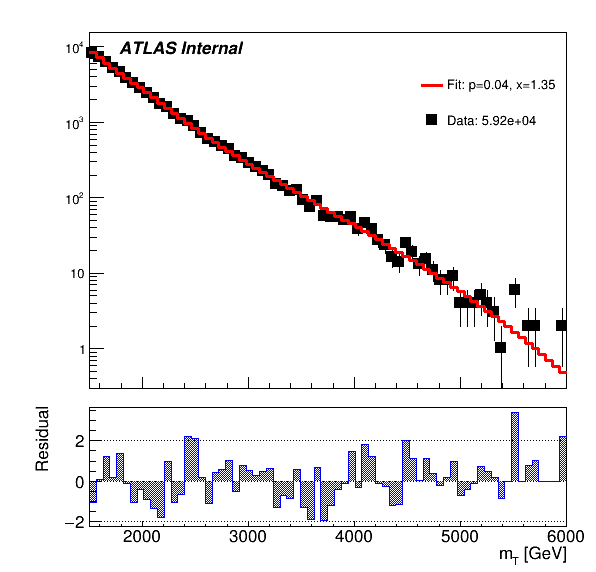
\includegraphics[width=0.32\textwidth]{figures/stats/dataDSfiveParFitChi2_VR2.png}
   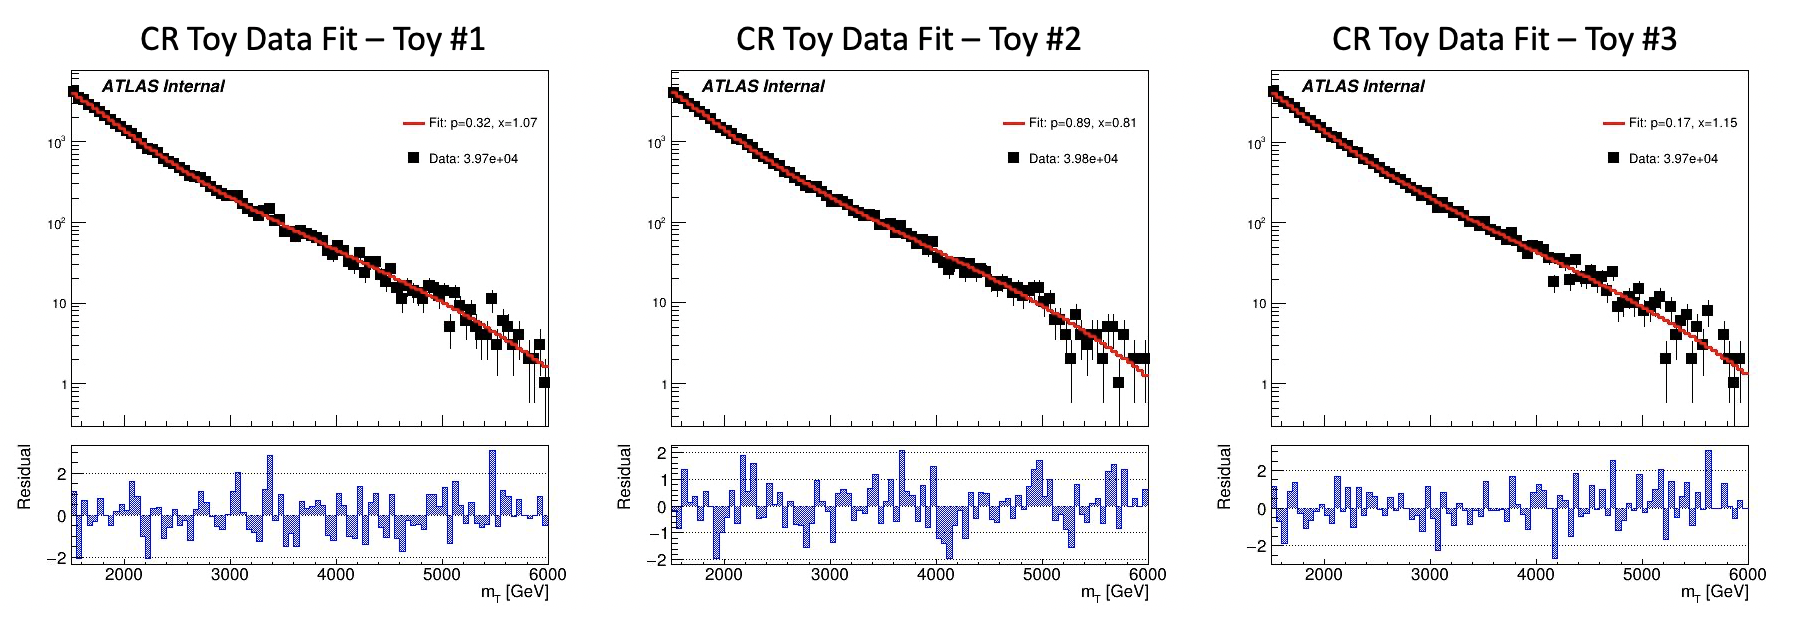
\includegraphics[width=0.97\textwidth]{figures/stats/bkgfit_data_cr}
    \caption{Background-only \mt~fits using pseudo-data from the CR template.
     \label{fig:bkgfit_data}}
\end{figure}

\begin{figure}[!htbp]
\centering
   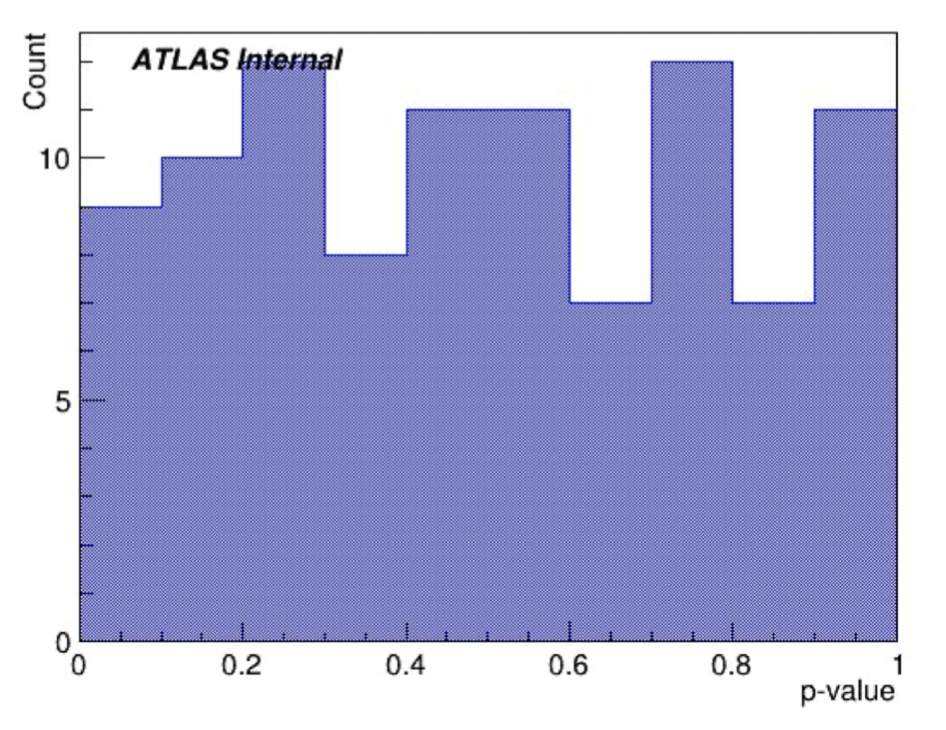
\includegraphics[width=0.6\textwidth]{figures/stats/asimov_cr_hist}
    \caption{$p$-value histograms from 100 fits to Asimov data in the CR. %, demonstrating a flat shape across p-value.
    \label{fig:asimov_hist}}
\end{figure}

\clearpage
%------------------------------------------------- 
\subsubsection{Signal + Background Fits}
\label{subsec:fit_splusb}

Figure~\ref{fig:splusb_sigInj} shows an example of an injected signal into the exclusion region \mt~spectrum, and the ability of the fit framework to accurately fit the number of signal events.
\begin{figure}[!htbp]
\centering
   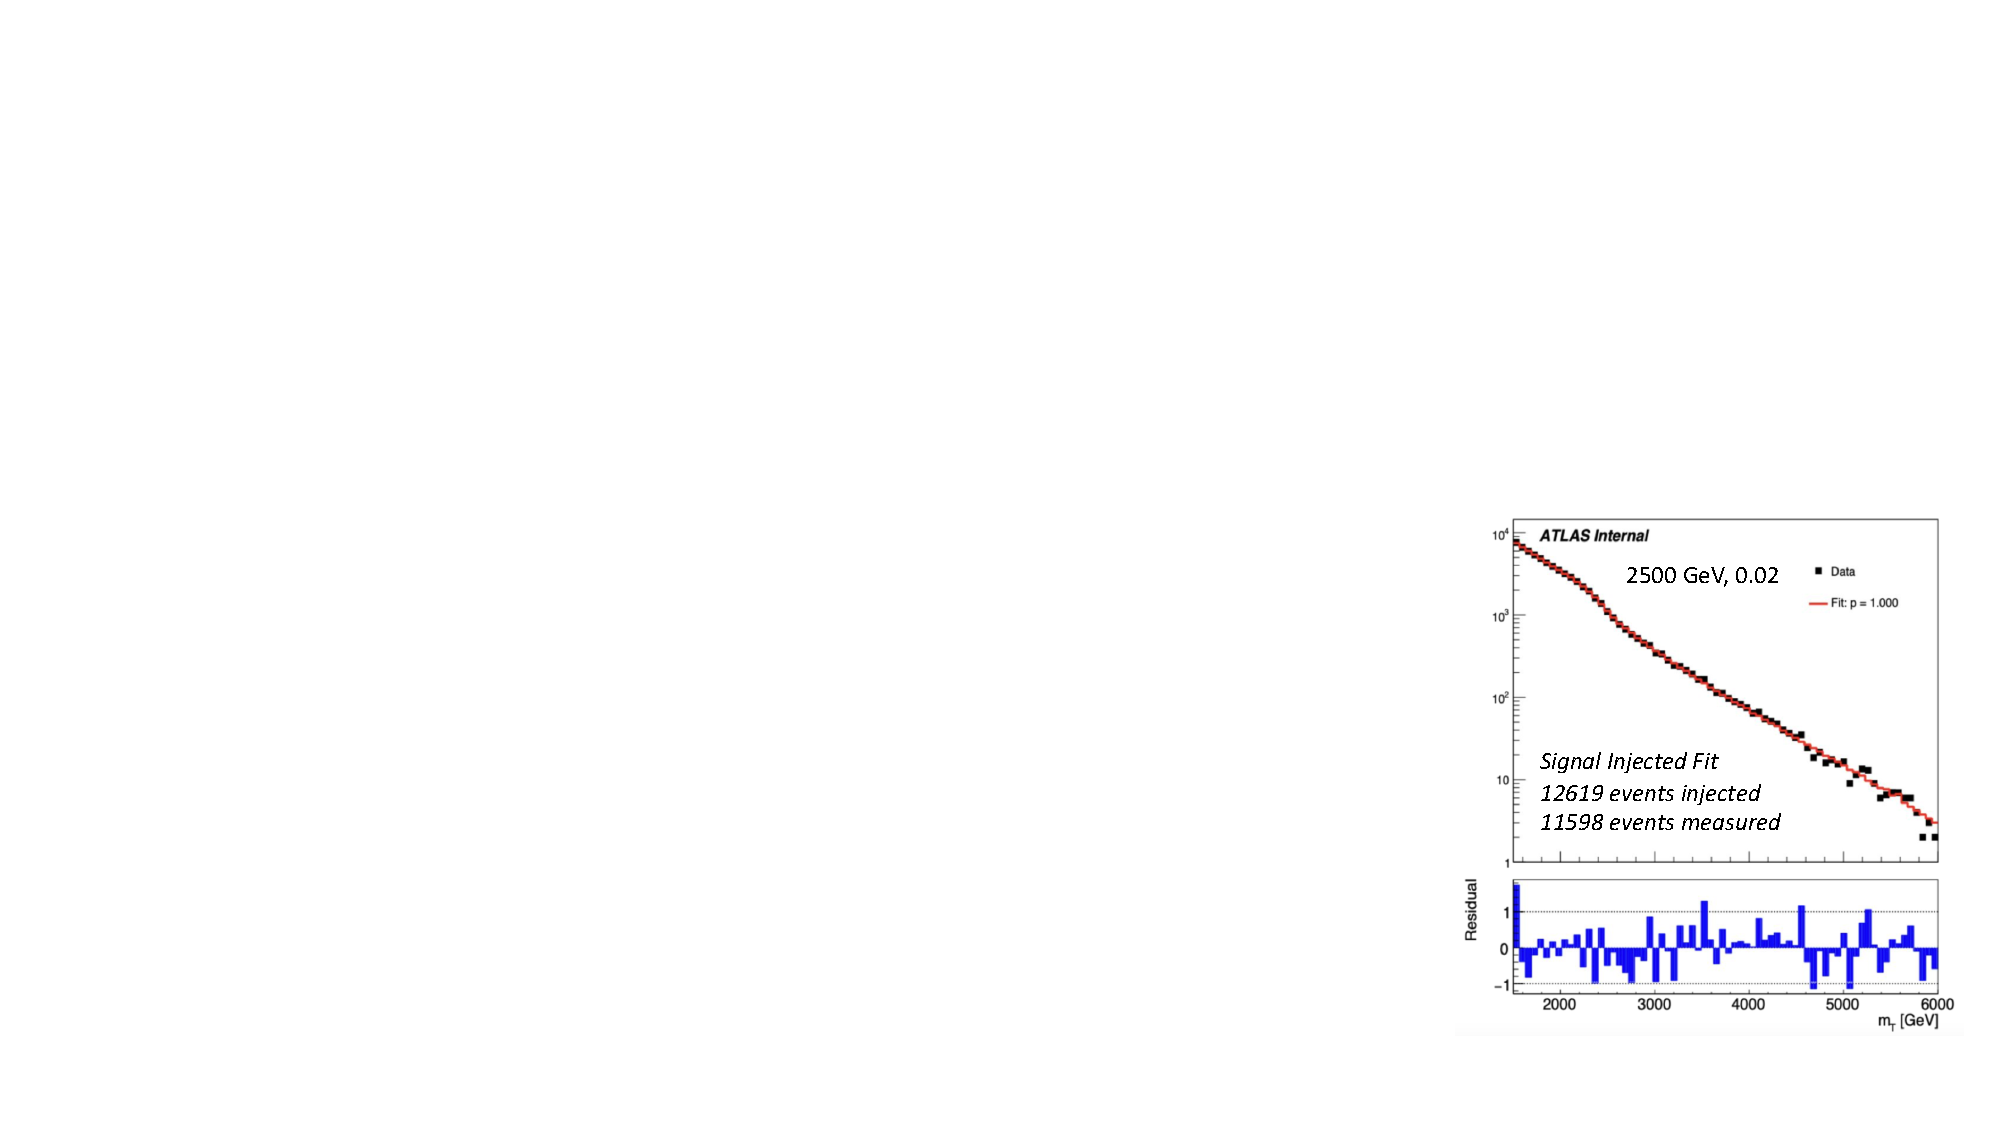
\includegraphics[width=0.6\textwidth]{figures/stats/splusb_sigInj}
    \caption{Example S+B fit on a background \mt~spectrum with injected signal from the point (4000 GeV, \rinv=0.2).
    \label{fig:splusb_sigInj}}
\end{figure}

Signal injection tests demonstrate the a linear relationship between the amount of signal injected and the amount of signal measured by the fit.
The signal injection tests are performed in Asimov datasets to counter the impact of statistical fluctuations in any given template.
50 Asimov trials are run for all signal points across Z' mass and \rinv.

%Bias within the Asimov signal injection test could indicate a lack of sufficient normalization uncertainties on the signal model. 
%In the event of systematic mismeasurement in signal injection, the spurious signal uncertainty as derived from Loose-not-tight or additional uncertainties will be considered.

Figure~\ref{fig:siginj_asimov} provides the results of these tests. 
The uncertainty of the measurement varies according to the Z' mass, due to the larger relative background for lower mass points. 
However, a strong linear relationship between amount of signal injected and amount of signal measured is observed for all signal points, which is the key feature.
\begin{figure}[!htbp]
\centering
   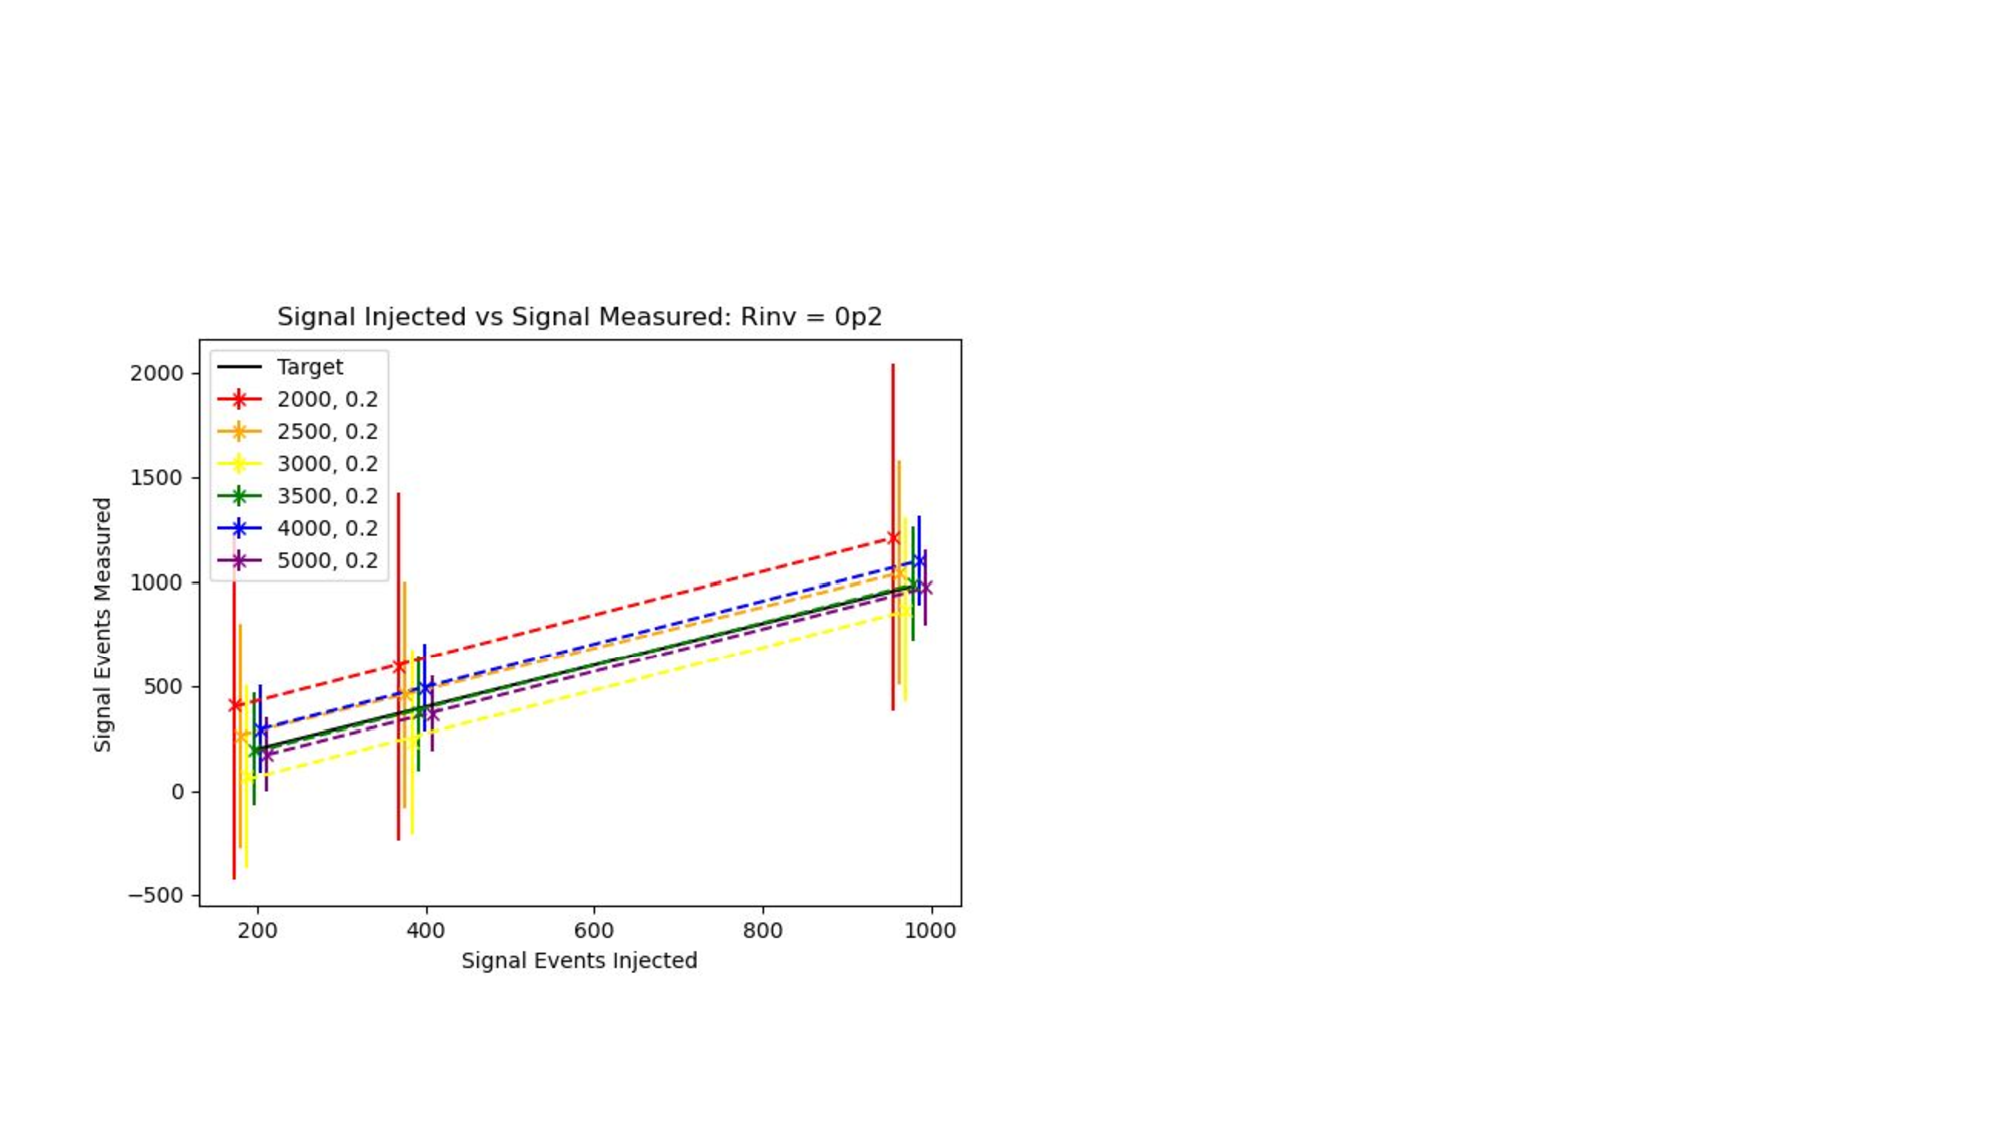
\includegraphics[width=0.45\textwidth]{figures/stats/siginj_asimov_02}
   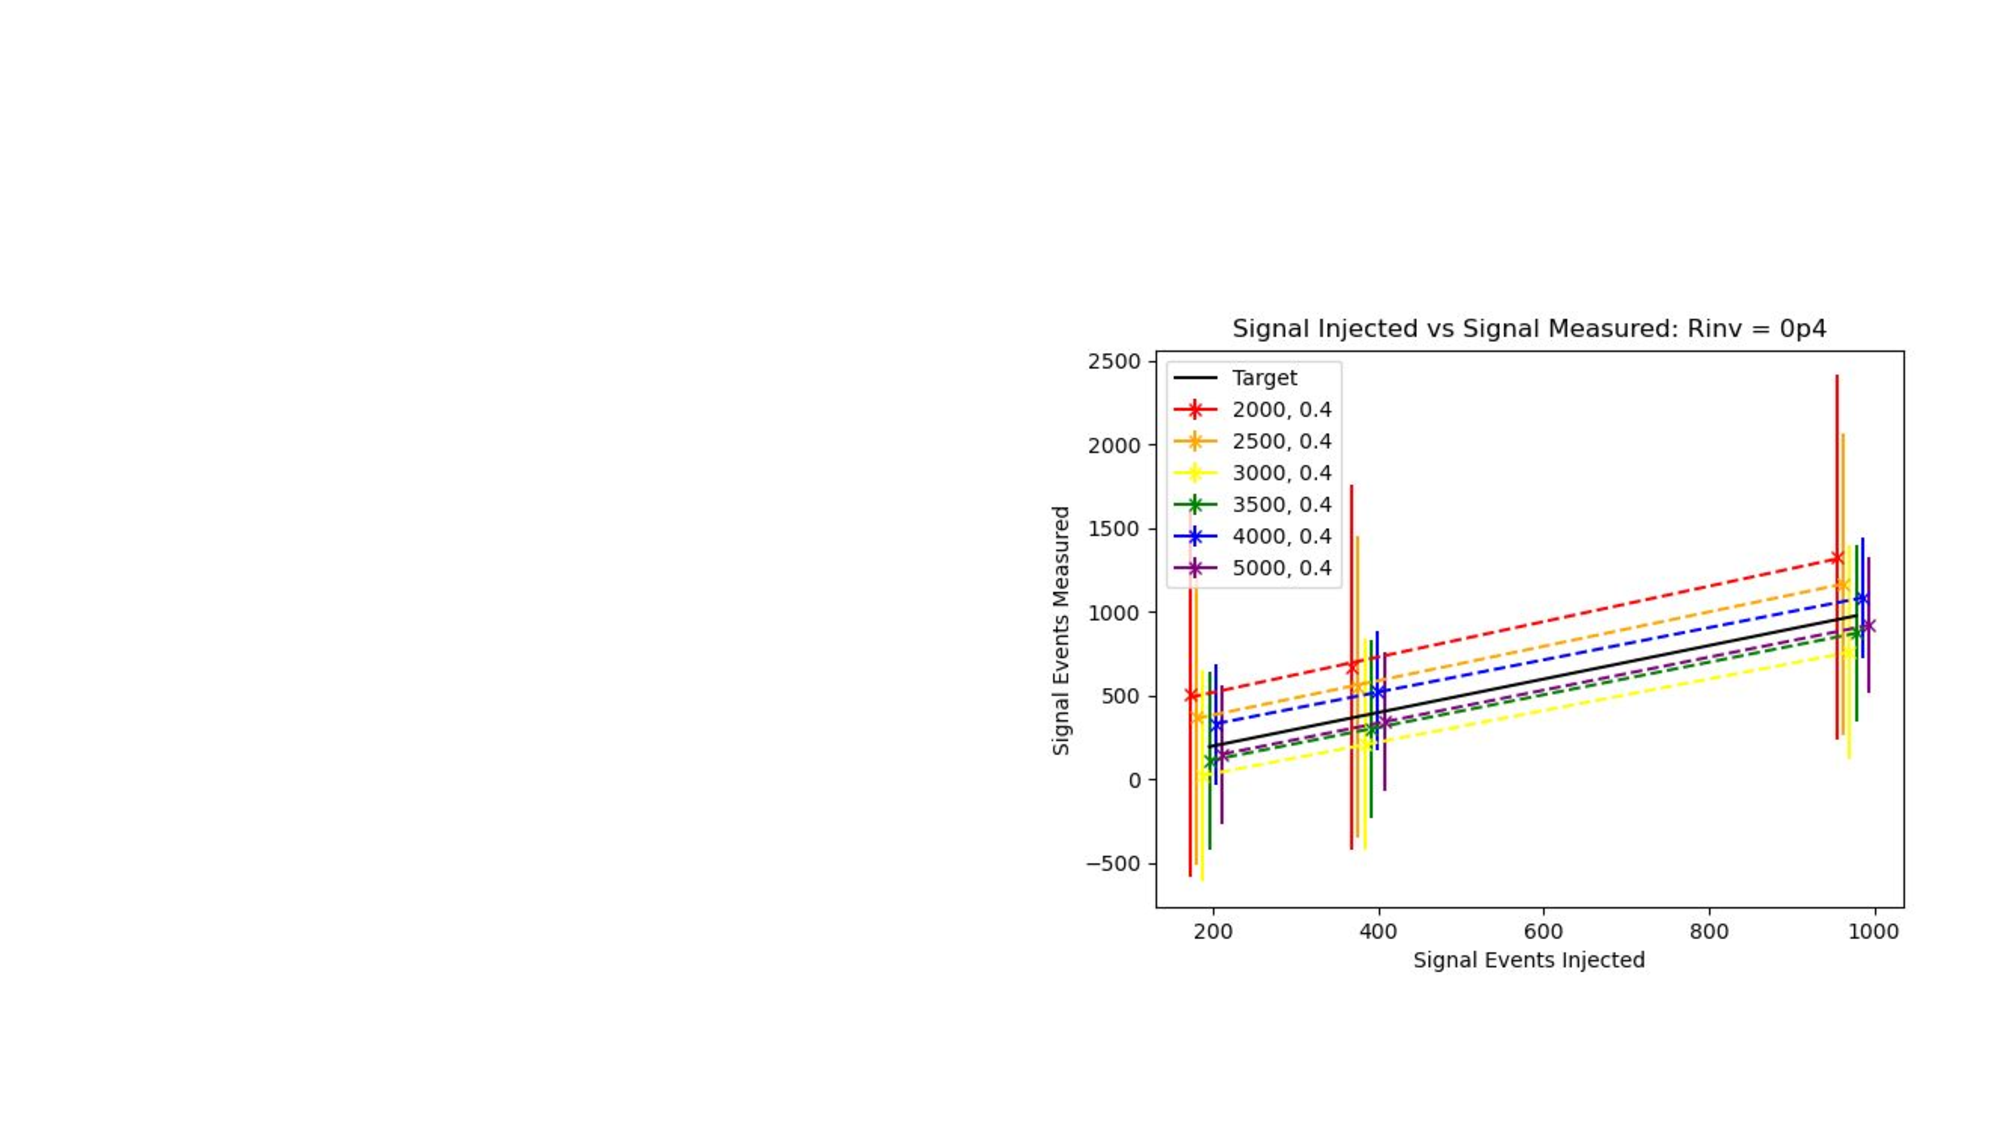
\includegraphics[width=0.45\textwidth]{figures/stats/siginj_asimov_04}
   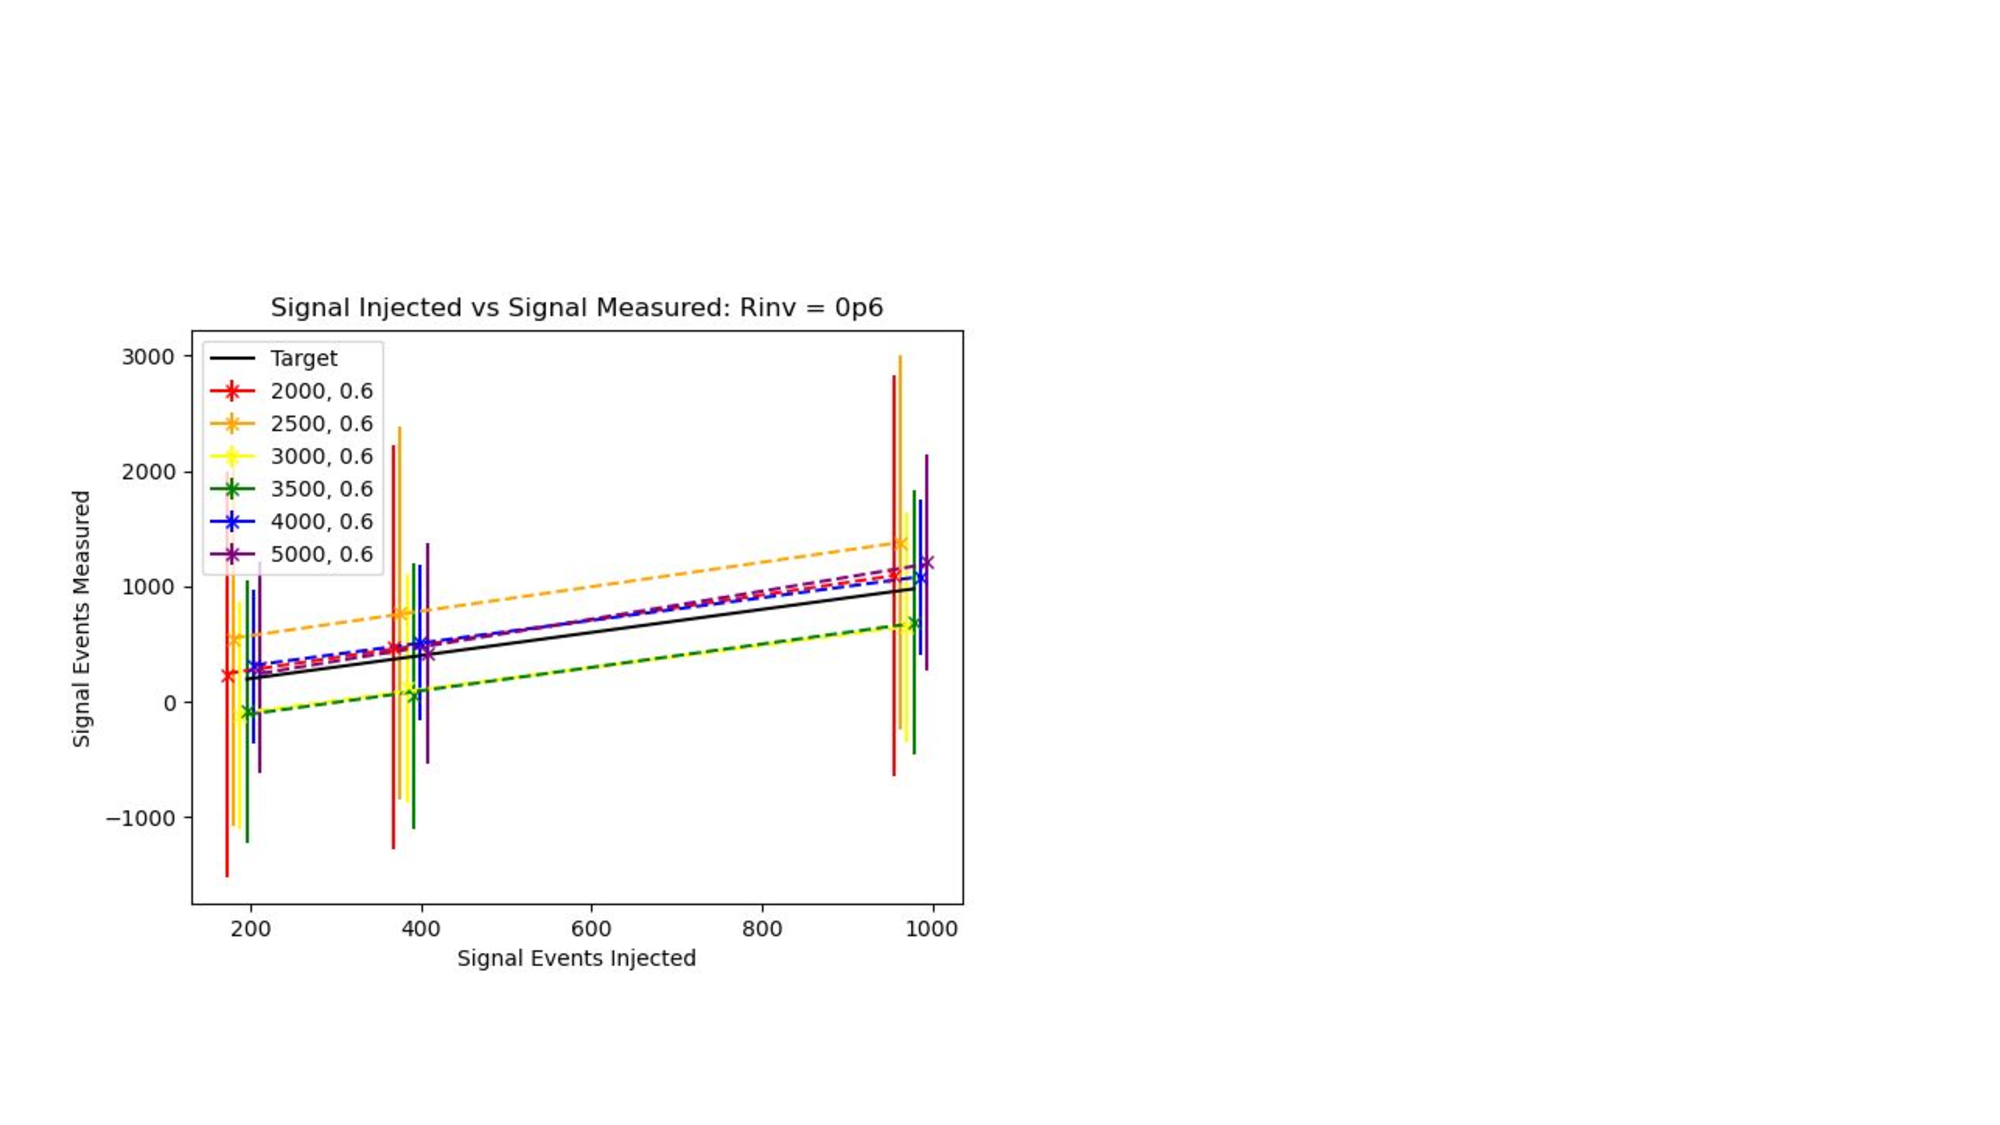
\includegraphics[width=0.45\textwidth]{figures/stats/siginj_asimov_06}
   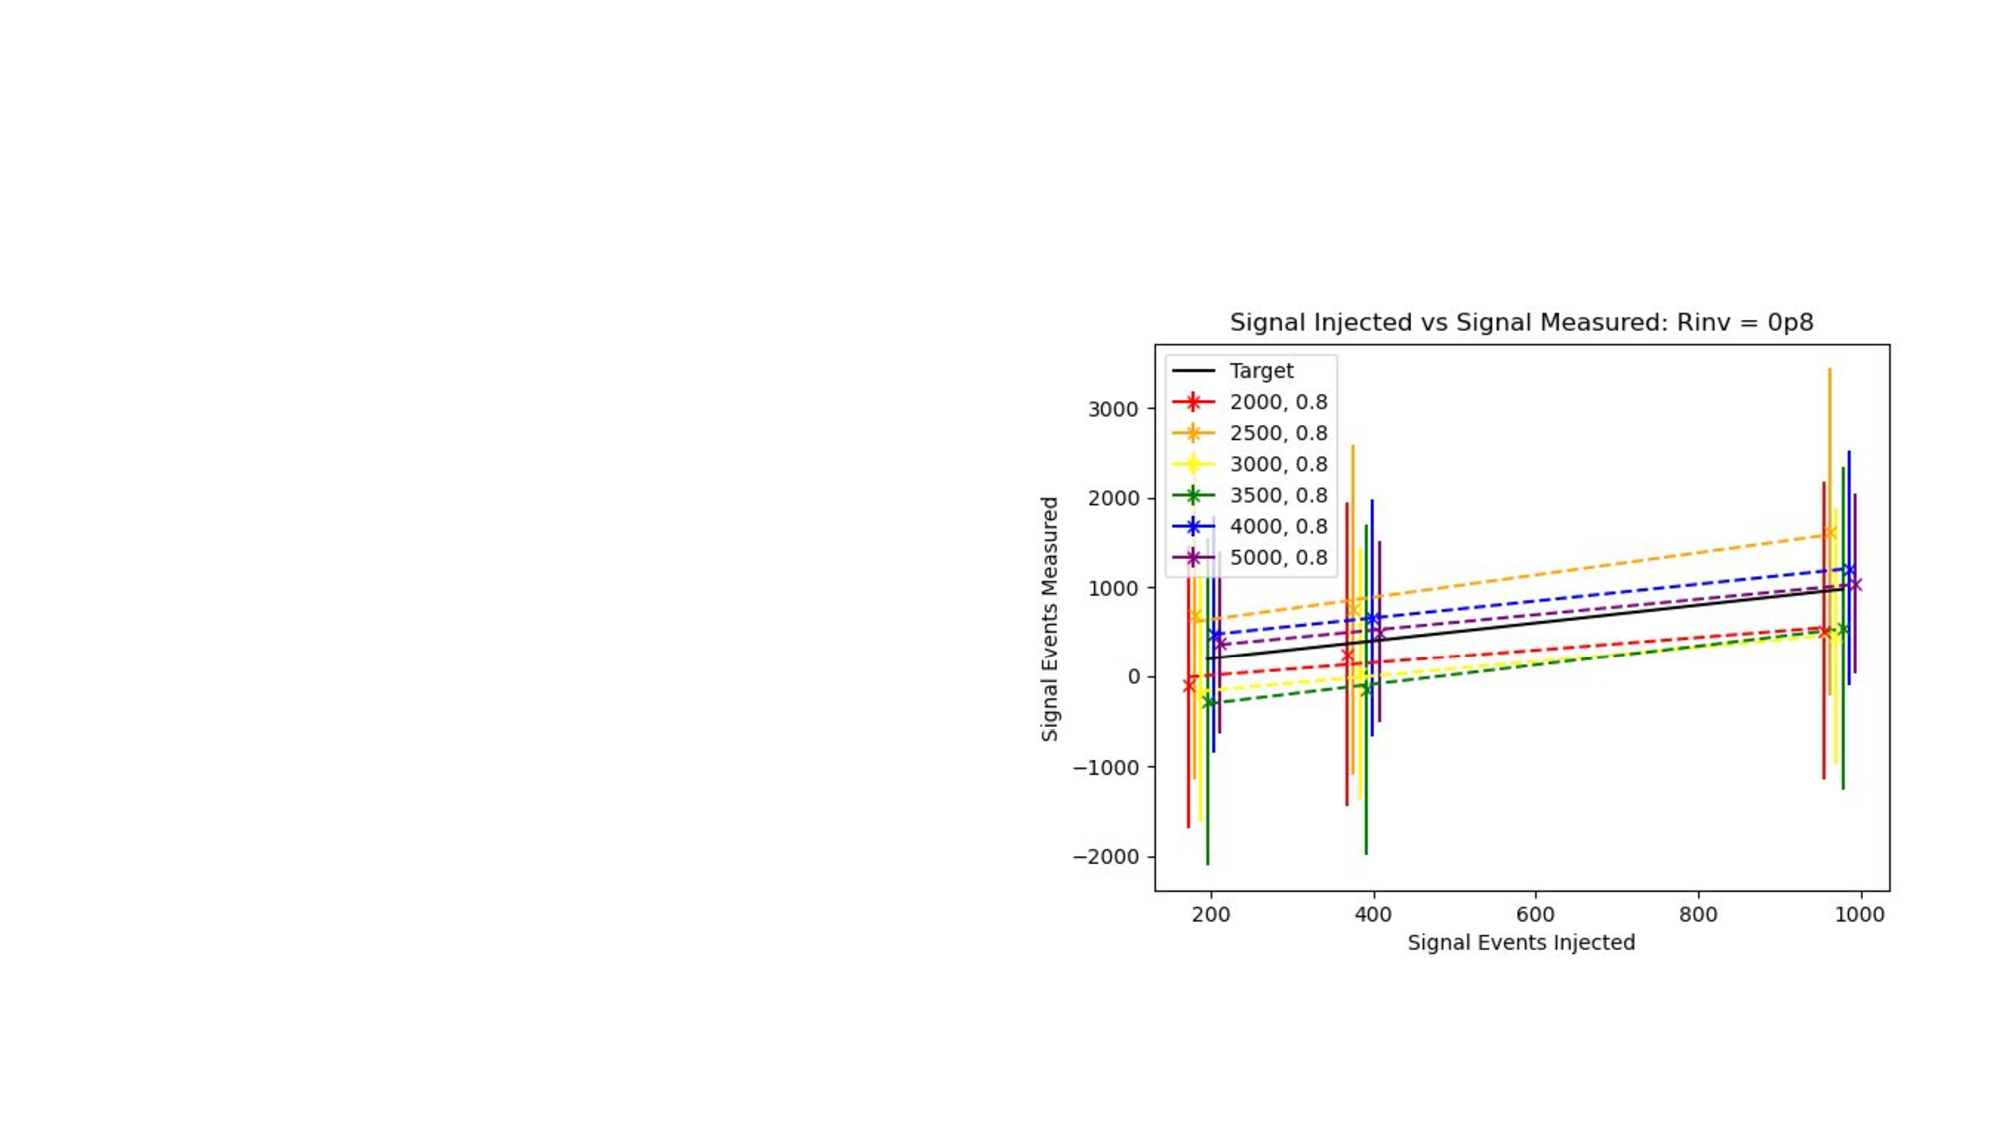
\includegraphics[width=0.45\textwidth]{figures/stats/siginj_asimov_08}
   \caption{Measured signal at a variety of injected values (1x, 2x, and 5x$\sqrt{b}$), for all signal points in the grid, \rinv=0.2 (top left), 0.4 (top right), 0.6 (bottom left), and 0.8 (bottom right).
%he requirement relative to $\sigma_{\text{fit}}$ is met for every signal point and injected signal size, thus satisfying the OR criteria from Equation~\ref{eq:spursig}.
    \label{fig:siginj_asimov}}
\end{figure}

\clearpage
%------------------------------------------------- 
\subsubsection{Expected Sensitivity}
\label{subsec:fit_expsens}

Limits on the signal process are obtained by determining the cross section of the signal that can be excluded to 95\% confidence. 
Figure~\ref{fig:limits_exp_1D} shows the expected limits obtained from an average of 50 Asimov data fits. The limits shown do not include systematics uncertainties in the fit, the impacts of which are discussed in Chaper~\ref{ch:results}. 
%Figure~\ref{fig:limits_exp_1D_asimov} shows the expected limits obtained from an average of 50 Asimov toys thrown from the CR.
%The limits are very stable across individual data fits and Asimov, as well as across the CR and VR.
%The alignment of fluctuations between the single CR fit and Asimov toys indicates that the particular shape of data in the CR influences the shape of the limits.
%The limits shown come from an average of 10 Asimov pseudodata fits of the CR. Figure~\ref{fig:perc_success_limit} shows the percentage of Asimov limit tests that result in a successful fit. 

Considerable exclusion power is predicted for low \rinv~signal points and lower mass points.
Higher \rinv~points present more difficulty due to the very broad signal bump.
Higher Z' mass points are more difficult to exclude due to the low theory cross-sections.

\begin{figure}[!htbp]
\centering
   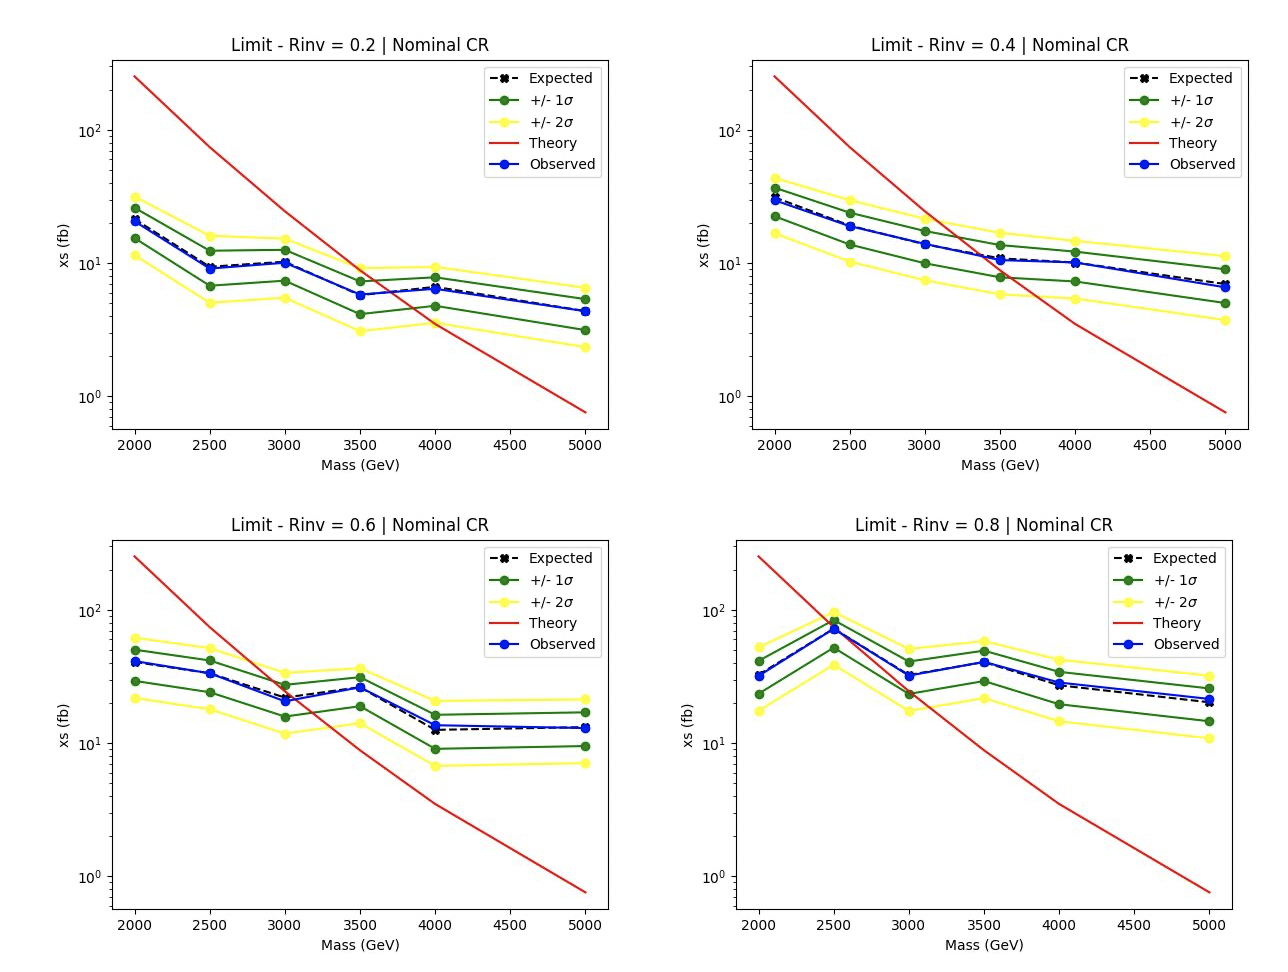
\includegraphics[width=0.95\textwidth]{figures/stats/limits_exp_1D}
    \caption{95\% C.L. upper limits for signal models across Z' mass, for four different \rinv~fractions, from the CR region (without systematics). TODO - ATLAS style
    \label{fig:limits_exp_1D}}
\end{figure}
%\begin{figure}[!htbp]
%\centering
%   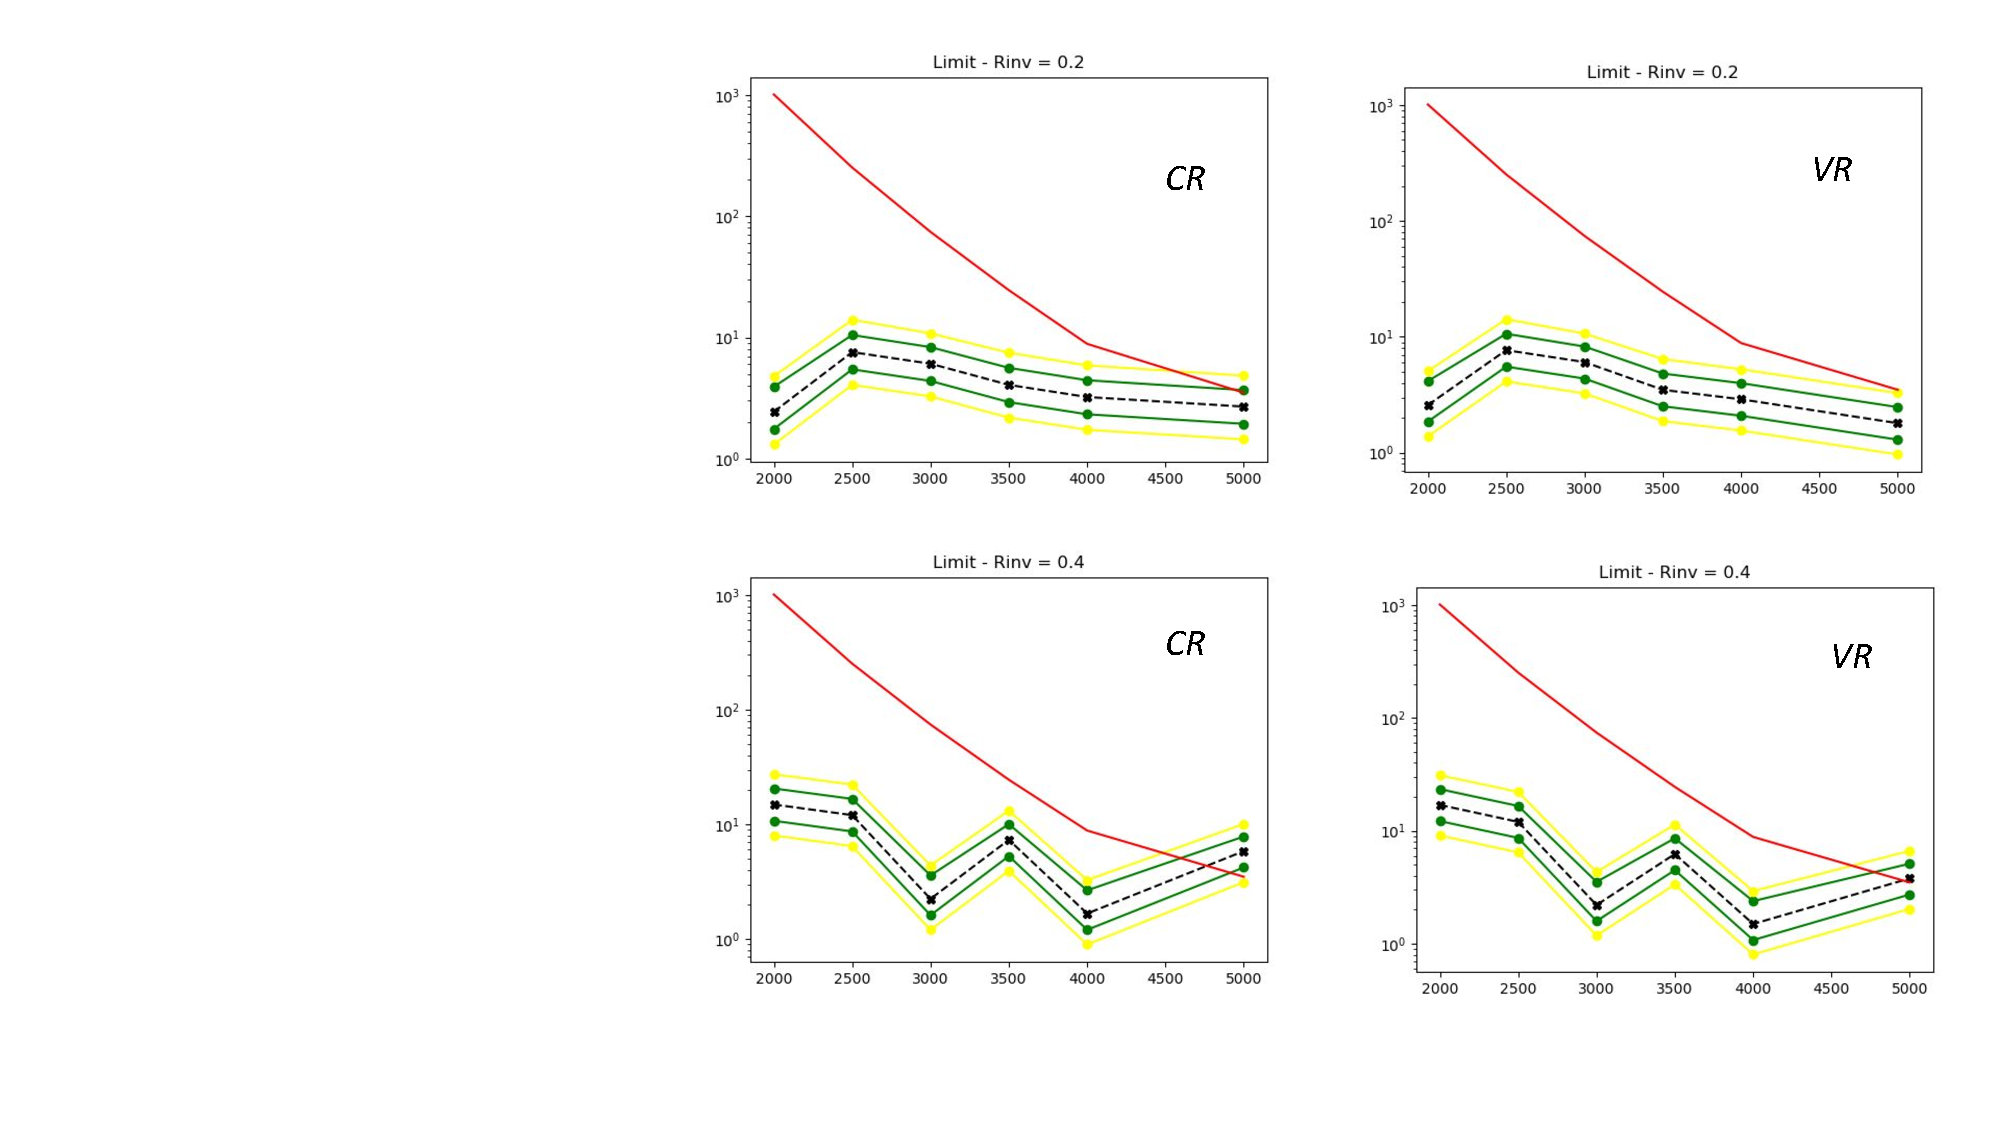
\includegraphics[width=0.9\textwidth]{figures/stats/limits_exp_1D_asimov_1}
%   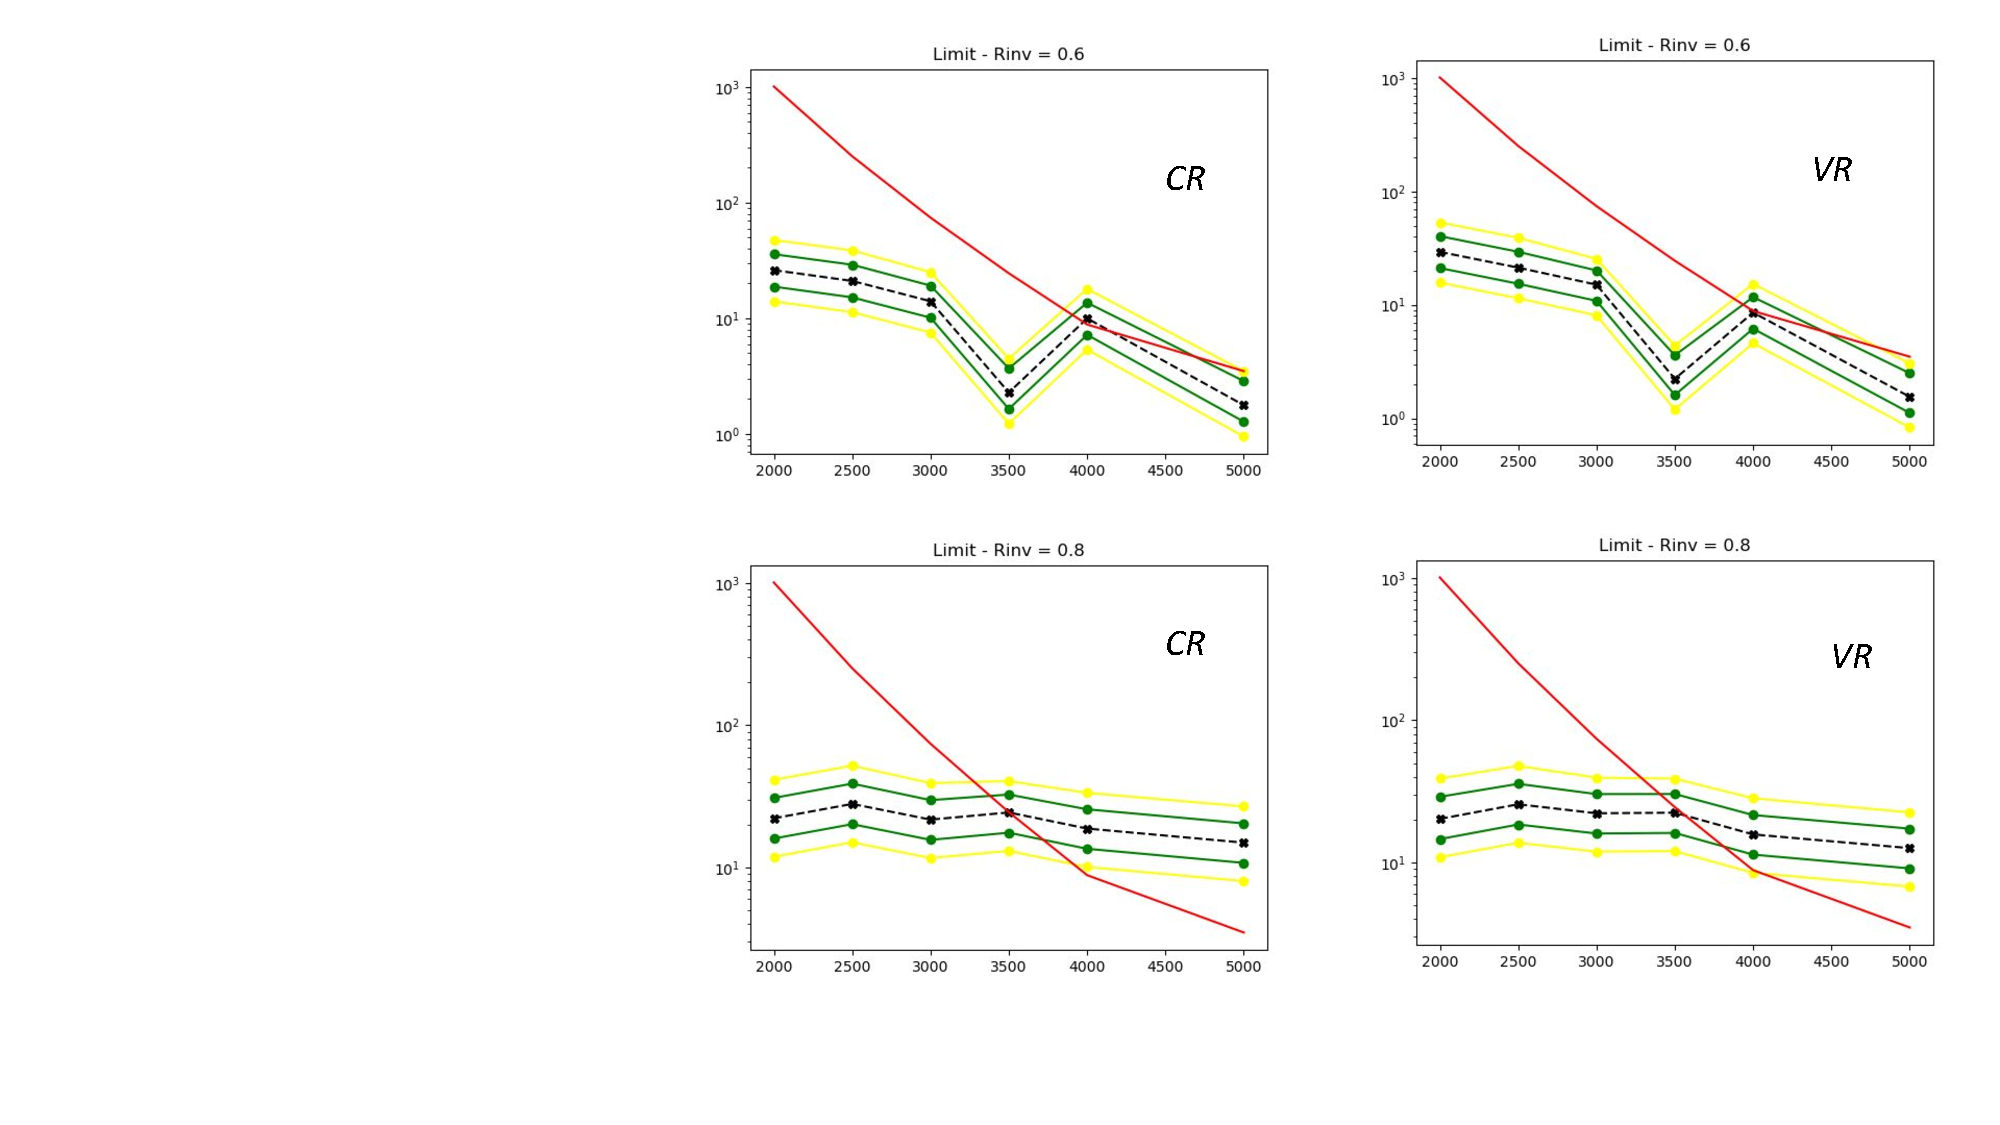
\includegraphics[width=0.9\textwidth]{figures/stats/limits_exp_1D_asimov_2}
%    \caption{95\% C.L. upper limits for signal models across Z' mass, for four different \rinv~fractions, using an average of 50 Asimov pseudo-data tests from the CR (left) and VR (right) (without systematics).
%    \label{fig:limits_exp_1D_asimov}}
%\end{figure}

%\begin{figure}[!htbp]ß
%\centering
%   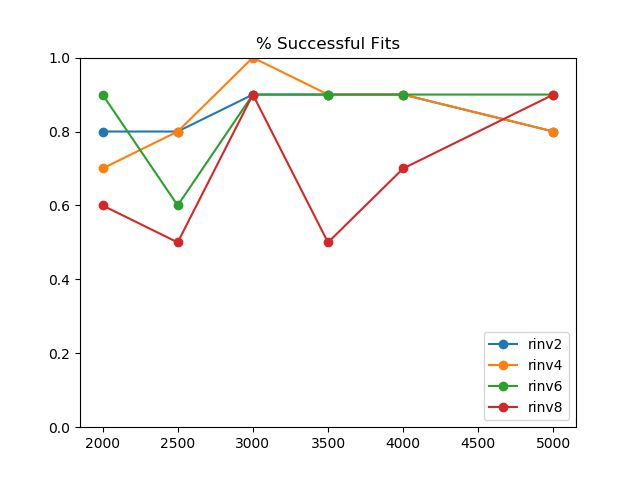
\includegraphics[width=0.6\textwidth]{figures/stats/perc_success_limit}
%    \caption{Percent of Asimov pseudodata S+B fits with successful fit and successful limit convergence.
%    \label{fig:perc_success_limit}}
%\end{figure}

The ability of the fit to identify is a significant excess is tested by calculating the limits on signal injected toys. $2\sigma$ and $5\sigma$ of signal is injected for each signal point into 50 Asimov data toys.
%The number of signal events necessary for a $2\sigma$/ $5\sigma$ excess is calculated for each signal point from the expected limits in the background-only case shown in Figure~\ref{fig:limits_exp_1D}.
%The expected limit represents the limit on a $2\sigma$ excess, so a $5\sigma$ excess requires 2.5x as much signal.
Figure~\ref{fig:lim_sig_inj} demonstrates the impact of this signal injection on the limit for \rinv~= 0.2.
The observed limit rises as more signal is injected, indicating the ability of the fit to identify a significant signal excess. 

\begin{figure}[!htbp]
\centering
   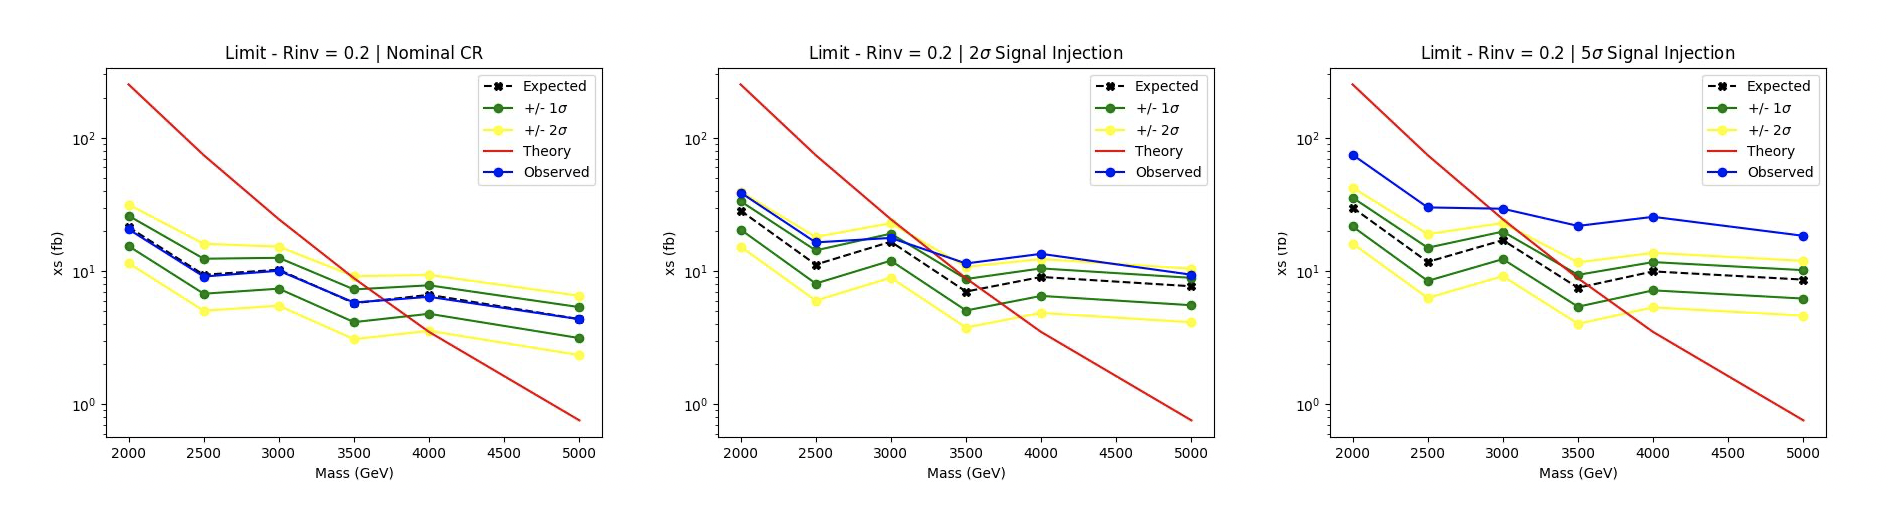
\includegraphics[width=0.98\textwidth]{figures/stats/lim_sig_inj}
    \caption{95\% C.L. upper limits and observed limit for signal models across Z' mass, with varying amounts of signal injected. TODO - ATLAS style
    \label{fig:lim_sig_inj}}
\end{figure}


